\documentclass[conference]{IEEEtran}
\IEEEoverridecommandlockouts
\usepackage{cite}
\usepackage{amsmath,amssymb,amsfonts}
\usepackage{algorithm}
\usepackage{algorithmic}
\usepackage{graphicx}
\usepackage{textcomp}
\usepackage{xcolor}
\usepackage[hyphens]{url}
\usepackage{tikz}
\usetikzlibrary{shapes.geometric,arrows.meta,positioning,backgrounds}
\tikzset{
  flowfont/.style={font=\footnotesize},
  startstop/.style={rectangle, rounded corners=3pt, draw=black!55, fill=black!8, thick, align=center, inner sep=4pt, minimum height=7mm},
  proc/.style={rectangle, rounded corners=3pt, draw=blue!60, fill=blue!8, thick, align=center, inner sep=4pt, minimum height=7mm},
  decide/.style={diamond, aspect=2.2, draw=orange!80!black, fill=orange!15, thick, align=center, inner sep=1pt},
  pick/.style={rectangle, rounded corners=3pt, draw=green!55!black, fill=green!14, thick, align=center, inner sep=4pt, minimum height=7mm},
  guard/.style={rectangle, rounded corners=3pt, draw=red!70!black, fill=red!8, thick, align=center, inner sep=4pt, minimum height=7mm},
  flowarr/.style={-{Latex[length=2mm]}, thick, draw=black!75},
  flbl/.style={font=\scriptsize\itshape, inner sep=1.5pt},
}
\def\BibTeX{{\rm B\kern-.05em{\sc i\kern-.025em b}\kern-.08em
    T\kern-.1667em\lower.7ex\hbox{E}\kern-.125emX}}
\begin{document}

\title{Efficient Polling-Based Learning Rate Optimization for Neural Networks}

\author{
\IEEEauthorblockN{Luiz Henrique}
\IEEEauthorblockA{\textit{} \\
\textit{Universidade Federal de Pernambuco} \\
Recife, Brazil \\
lhbas@cin.ufpe.br}
\and
\IEEEauthorblockN{Jos\'{e} Ronaldo}
\IEEEauthorblockA{\textit{} \\
\textit{Universidade Federal de Pernambuco} \\
Recife, Brazil \\
jrss@cin.ufpe.br}
}

\maketitle

\begin{abstract}
Selecting an appropriate learning rate is one of the most critical decisions in training neural networks effectively. This work has two objectives: (1) to replicate the Polling Method proposed by Tan et al.\ on the CIFAR-10 benchmark, adapting it from the original ANN setting to a convolutional neural network trained with SGD, and (2) to propose and evaluate a novel extension (the Efficient Polling method) against a fixed-rate SGD baseline over 150 epochs. The replicated Polling method dramatically surpasses the baseline, achieving 84.65\% best validation accuracy and 83.99\% test accuracy versus the baseline's 56.70\%, by autonomously selecting high learning rates early in training and transitioning to fine-grained steps near convergence. However, it pays a heavy price: every batch requires $N=5$ trial weight updates, more than tripling wall-clock training time. The proposed Efficient Polling method exploits the temporal stability of the selected learning rate by polling on demand: an exponential-backoff schedule doubles the interval between polls while the selection remains unchanged, and a two-tier divergence guard (spike-triggered polls and rollback to poll-point checkpoints) protects the unpolled steps. Efficient Polling matches the base method's accuracy (85.07\% best validation, 83.93\% test, within 0.1 pp) while polling only 5\% of batches, reducing optimizer steps by 75\% and wall-clock time per epoch by $3.3\times$, only 12\% slower than plain SGD. Our results confirm that polling-based selection is highly effective at learning rate discovery when candidates span the optimal range, and demonstrate that nearly all of its cost can be eliminated without sacrificing accuracy or robustness.
\end{abstract}

\begin{IEEEkeywords}
learning rate optimization, neural networks, polling method, CIFAR-10, efficient training, SGD optimizer
\end{IEEEkeywords}

\section{Introduction}

The learning rate (LR) is arguably the most influential hyperparameter in gradient-based training of neural networks. A rate that is too large causes divergence or oscillation near optima, while a rate that is too small leads to slow convergence or entrapment in poor local minima. Fixed learning rates require expert knowledge or costly grid search, motivating the development of adaptive strategies.

Existing approaches range from formula-based schedulers (step decay, cosine annealing~\cite{loshchilov2017sgdr}, ReduceLROnPlateau) to optimizers with built-in per-parameter adaptation such as Adam~\cite{kingma2015adam} and RMSProp~\cite{tieleman2012rmsprop}. A fundamentally different paradigm is \emph{polling optimization}, introduced by Tan et al.~\cite{tan2025polling}: rather than computing a single LR-scaled update, multiple candidate learning rates are tested at each gradient step and the one that most improves performance on the current batch is selected. This exploration-based approach requires no hand-designed formula and adapts implicitly to the loss landscape.

This work pursues two goals. First, we replicate the Polling Method on CIFAR-10, adapting it from the original ANN and MNIST setting to a convolutional neural network trained with SGD, a setup that differs from the original in architecture and candidate LR range. Second, we address the method's main weakness, its computational cost, by proposing the Efficient Polling method, which polls on demand instead of at every batch, and we compare all three strategies against a fixed-rate SGD baseline. We report training dynamics, convergence speed, generalization accuracy, and computational cost across 150 epochs.

\section{Proposed Solution}

\subsection{Background: Exploration vs.\ Exploitation}

Adaptive learning-rate methods are commonly framed as balancing two opposing goals. \emph{Exploitation} makes cautious, formula-bounded adjustments to converge efficiently toward a nearby minimum; \emph{exploration} makes larger, deliberate changes to escape poor local minima. Tan et al.\ argue that the dominant optimizers (SGD, RMSProp, and Adam) are primarily exploitation-driven: they attenuate the learning rate through fixed heuristic functions and accumulate gradient history through moving averages, which both bounds their adaptability and injects noise that can obscure the true gradient. Cyclic and warm-restart schedules~\cite{smith2017cyclical, loshchilov2017sgdr} add exploration, but still within a predefined functional form, so the learning rate can never move outside what that form allows.

The Polling Method was introduced to inject exploration into otherwise exploitation-based training without relying on any such formula. Rather than computing one learning-rate-scaled update, it instantiates an ensemble of $n$ \emph{base models} from the same weights, each advanced by a different candidate learning rate $\alpha_1, \ldots, \alpha_n$. Every base model is evaluated against the training labels, and the candidate that yields the highest-accuracy model is selected; its weights become the starting point for the next iteration, and the procedure repeats. Because the choice is driven by measured performance rather than a schedule, the method can raise the learning rate aggressively when that helps and lower it when it does not, exploring the learning-rate space continuously and eliminating any dependence on past gradients. Tan et al.\ validated the method with the Adam optimizer on Artificial Neural Networks and on a Bayesian variational-inference task, reporting a 50\% reduction in absolute error over Adam alone. Our work isolates this selection mechanism on top of vanilla SGD, removing Adam's per-parameter adaptation so that the polled learning rate is the only adaptive component, and moves the selection granularity to the mini-batch, as detailed next.

\subsection{Replicated Method: Polling}

The Polling Method, proposed by Tan et al., replaces the standard single-LR gradient step with an ensemble selection procedure. At every training batch, after computing gradients, $N$ candidate learning rates are applied independently and the model weights that achieve the highest batch accuracy are retained.

Let $\mathcal{C} = \{lr_1, \ldots, lr_N\}$ be the candidate set. At batch $t$, given weights $\theta_t$ and gradients $g_t$:
\begin{equation}
\hat{\theta}_{t,k} = \theta_t - lr_k \cdot g_t, \quad k = 1,\ldots,N
\end{equation}
\begin{equation}
k^{*} = \arg\max_{k} \; \mathrm{acc}(\hat{\theta}_{t,k},\, \mathcal{B}_t)
\end{equation}
\begin{equation}
\theta_{t+1} = \hat{\theta}_{t,k^{*}}
\end{equation}

where $\mathcal{B}_t$ is the current mini-batch. We use $\mathcal{C} = \{10^{-5},\, 10^{-4},\, 10^{-3},\, 10^{-2},\, 10^{-1}\}$, spanning five orders of magnitude centered around the base LR $= 10^{-3}$. Note that Tan et al.\ originally used LRs in the range $[0.01, 0.05]$ with a simple ANN and SGD-like updates; our candidate set is adapted to the CNN setting and covers a wider range to allow the optimizer to discover the most suitable LR autonomously.

Algorithm~\ref{alg:polling} states the per-batch procedure, and Fig.~\ref{fig:polling-flow} depicts the corresponding data flow. The selection requires $N$ trial weight updates evaluated from the same snapshot $(\theta_t, g_t)$; the winning candidate is kept directly, so no re-application step is needed. Ties on batch accuracy are broken in favor of the smallest candidate LR, matching the conservative behavior of the original method.

\begin{algorithm}[htbp]
\caption{Polling step (base method, one batch)}
\label{alg:polling}
\begin{algorithmic}[1]
\REQUIRE weights $\theta$, batch $\mathcal{B}$, candidate set $\mathcal{C}$, loss $L$
\STATE $g \leftarrow \nabla_\theta L(\theta; \mathcal{B})$ \COMMENT{gradient at current point}
\FOR{each $lr_k \in \mathcal{C}$}
    \STATE $\hat{\theta}_k \leftarrow \theta - lr_k \cdot g$ \COMMENT{trial step from snapshot}
    \STATE $a_k \leftarrow \mathrm{acc}(\hat{\theta}_k, \mathcal{B})$
\ENDFOR
\STATE $k^{*} \leftarrow \arg\max_k a_k$ \COMMENT{ties favor smallest $lr$}
\STATE $\theta \leftarrow \hat{\theta}_{k^{*}}$
\STATE \textbf{return} updated weights $\theta$, selected $lr^{*} = lr_{k^{*}}$
\end{algorithmic}
\end{algorithm}

In practice, the $N$ trial updates of line~3 are realized by deep-copying the model and optimizer states once, then, for each candidate, reloading that snapshot, overwriting the optimizer's learning rate, and taking a single optimizer step. Reloading the optimizer state alongside the weights guarantees that every candidate departs from the identical pre-step condition; for vanilla SGD without momentum the optimizer carries no state, so the restoration is exact and the selection is determined purely by the candidate learning rate. The selection criterion is the per-batch classification accuracy of the resulting weights on the same mini-batch $\mathcal{B}_t$ that produced the gradient, evaluated under \texttt{torch.no\_grad}~\cite{paszke2019pytorch}; cross-entropy is the training loss but accuracy is the selection signal, matching the original method's use of base-model accuracy. This snapshot-and-restore procedure is shared verbatim by Efficient Polling, where the snapshot taken at each poll is additionally retained as the rollback checkpoint used by the divergence guard.

\begin{figure}[htbp]
\centering
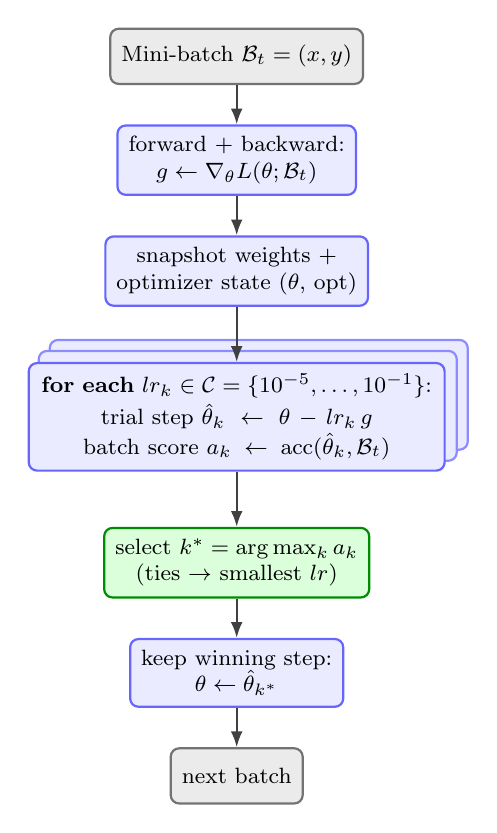
\begin{tikzpicture}[node distance=5mm, flowfont]
  \node[startstop] (b) {Mini-batch $\mathcal{B}_t=(x,y)$};
  \node[proc, below=of b] (grad) {forward $+$ backward:\\$g \leftarrow \nabla_\theta L(\theta;\mathcal{B}_t)$};
  \node[proc, below=of grad] (snap) {snapshot weights $+$\\optimizer state $(\theta,\,\mathrm{opt})$};
  \node[proc, below=7mm of snap, text width=50mm] (trial) {\textbf{for each} $lr_k \in \mathcal{C}=\{10^{-5},\dots,10^{-1}\}$:\\[1pt]trial step $\hat\theta_k \leftarrow \theta - lr_k\,g$\\[1pt]batch score $a_k \leftarrow \mathrm{acc}(\hat\theta_k,\mathcal{B}_t)$};
  \node[pick, below=7mm of trial] (sel) {select $k^{*}=\arg\max_k a_k$\\(ties $\rightarrow$ smallest $lr$)};
  \node[proc, below=of sel] (keep) {keep winning step:\\$\theta \leftarrow \hat\theta_{k^{*}}$};
  \node[startstop, below=of keep] (next) {next batch};
  \begin{scope}[on background layer]
    \draw[draw=blue!45, fill=blue!8, thick, rounded corners=3pt]
      ([xshift=2.8mm,yshift=2.8mm]trial.south west) rectangle ([xshift=2.8mm,yshift=2.8mm]trial.north east);
    \draw[draw=blue!45, fill=blue!8, thick, rounded corners=3pt]
      ([xshift=1.4mm,yshift=1.4mm]trial.south west) rectangle ([xshift=1.4mm,yshift=1.4mm]trial.north east);
  \end{scope}
  \draw[flowarr] (b) -- (grad);
  \draw[flowarr] (grad) -- (snap);
  \draw[flowarr] (snap) -- (trial);
  \draw[flowarr] (trial) -- (sel);
  \draw[flowarr] (sel) -- (keep);
  \draw[flowarr] (keep) -- (next);
\end{tikzpicture}
\caption{Per-batch control flow of the base Polling method (Algorithm~\ref{alg:polling}). Each batch computes a single gradient, then evaluates all $N$ candidate learning rates as trial steps from the same snapshot and keeps the weights with the highest batch accuracy. The stacked block denotes the $N$ independent trial updates.}
\label{fig:polling-flow}
\end{figure}

\subsection{Proposed Extension: Efficient Polling}

The base Polling method performs $N$ trial weight updates at \emph{every} batch, yet its selection is highly redundant: within each phase of training, consecutive polls overwhelmingly choose the same learning rate. The Efficient Polling method keeps the selection mechanism of base Polling untouched but polls \emph{on demand}, combining an adaptive polling schedule with a divergence guard for the unpolled steps.

\subsubsection{Adaptive polling schedule}
Let $K$ be the current polling interval, in batches. A batch is polled when $K$ batches have elapsed since the last poll; all other batches perform a single standard SGD step using the last selected learning rate. After each poll, $K$ is updated by exponential backoff:
\begin{equation}
K \leftarrow
\begin{cases}
\min(2K,\; K_{\max}) & \text{if } lr^{*} = lr^{*}_{\mathrm{prev}} \\
1 & \text{otherwise}
\end{cases}
\label{eq:backoff}
\end{equation}
where $lr^{*}$ is the LR selected by the poll. A stable selection therefore decays the polling frequency geometrically (up to one poll every $K_{\max}$ batches), while any change in the selection immediately restores per-batch polling until the choice stabilizes again. Backoff only engages after the first poll in which candidate accuracies differ: at initialization all candidates tie on batch accuracy, and treating those ties as ``stable'' would stall training at the minimum candidate LR.

\subsubsection{Divergence guard}
Unlike base Polling, which evaluates every step before keeping it, Efficient Polling applies the steps between polls blindly. At a high learning rate, a single batch with a large gradient can then push the weights into divergence with no opportunity for the poll to reject the step. The guard exploits the pre-step batch loss $\ell_t$, which is already computed for the gradient, and operates at two tiers:

\paragraph{Spike-triggered polls (prevention)} An exponential moving average of the batch loss, $\bar{\ell}_t = \beta\,\bar{\ell}_{t-1} + (1-\beta)\,\ell_t$, tracks the current loss level. If a batch arrives with $\ell_t > \gamma\,\bar{\ell}_{t-1}$, it is polled immediately regardless of the schedule, so that the accuracy criterion can reject an explosive step before it is applied.

\paragraph{Rollback checkpoints (recovery)} The model and optimizer states stored by each poll double as a checkpoint of the last known-good weights. If $\ell_t$ is non-finite or exceeds an absolute threshold $\ell_{\mathrm{rb}} = 2\ln C$ (twice the cross-entropy loss of random guessing over $C$ classes), the weights are considered broken: the checkpoint is restored, the step is skipped, and polling resumes on the next batch. At most $K_{\max}$ batches of progress are lost.

The full configuration is given in Table~\ref{tab:config}; the candidate set is identical to base Polling, and the four guard/backoff constants are the only quantities Efficient Polling adds over the base method.

\begin{table}[htbp]
\caption{Efficient Polling Configuration}
\begin{center}
\resizebox{\columnwidth}{!}{%
\begin{tabular}{|l|c|l|}
\hline
\textbf{Symbol} & \textbf{Value} & \textbf{Role} \\
\hline
$\mathcal{C}$            & $\{10^{-5},\ldots,10^{-1}\}$ & candidate learning rates \\
$lr_{\mathrm{init}}$     & $10^{-3}$        & LR before the first poll \\
$K_{\max}$               & $64$             & max poll interval (backoff cap) \\
$\gamma$                 & $3$              & spike threshold (tier 2) \\
$\beta$                  & $0.9$            & loss-EMA decay \\
$\ell_{\mathrm{rb}}$     & $2\ln 10 \approx 4.61$ & rollback threshold (tier 1) \\
\hline
\end{tabular}%
}
\end{center}
\label{tab:config}
\end{table}

Algorithm~\ref{alg:efficient} assembles these components into the per-epoch training loop, and Fig.~\ref{fig:eff-flow} shows the resulting per-batch control flow. The poll itself reuses the selection of Algorithm~\ref{alg:polling}; because the trial updates overwrite the weights, the winning step is re-applied once after selection (a single extra optimizer step per poll, accounted for in Section~\ref{sec:cost}). Every poll also refreshes the rollback checkpoint, so the recovery tier carries no additional bookkeeping.

\begin{algorithm}[htbp]
\caption{Efficient Polling (one epoch)}
\label{alg:efficient}
\begin{algorithmic}[1]
\REQUIRE loader, candidate set $\mathcal{C}$, params $K_{\max}, \gamma, \beta, \ell_{\mathrm{rb}}$
\STATE $K \leftarrow 1$,\; $s \leftarrow 1$,\; $lr^{*} \leftarrow lr_{\mathrm{init}}$ \COMMENT{persisted across epochs}
\STATE $\bar{\ell} \leftarrow \textsc{None}$,\; $\theta_{\mathrm{ck}} \leftarrow \textsc{None}$,\; \texttt{seen} $\leftarrow$ \textsc{False}
\FOR{each batch $\mathcal{B} = (x,y)$}
    \STATE $\ell \leftarrow L(\theta; \mathcal{B})$
    \IF{$\ell$ is non-finite \textbf{ or } $\ell > \ell_{\mathrm{rb}}$}
        \STATE restore $\theta \leftarrow \theta_{\mathrm{ck}}$;\; $K \leftarrow 1$;\; $s \leftarrow 1$ \COMMENT{tier 1: rollback}
        \STATE \textbf{continue}
    \ENDIF
    \STATE $g \leftarrow \nabla_\theta \ell$
    \STATE $\mathit{spike} \leftarrow (\bar{\ell} \neq \textsc{None}) \wedge (\ell > \gamma\,\bar{\ell})$ \COMMENT{tier 2}
    \IF{$\mathit{spike}$ \textbf{ or } $s \geq K$}
        \STATE $(lr_{\mathrm{new}}, \mathit{signal}) \leftarrow \textsc{Poll}(\theta, \mathcal{B}, \mathcal{C})$
        \IF{\textbf{not} \texttt{seen}}
            \STATE \texttt{seen} $\leftarrow \mathit{signal}$;\; $K \leftarrow 1$
        \ELSIF{$lr_{\mathrm{new}} = lr^{*}$}
            \STATE $K \leftarrow \min(2K,\, K_{\max})$ \COMMENT{backoff}
        \ELSE
            \STATE $K \leftarrow 1$ \COMMENT{selection changed: poll again}
        \ENDIF
        \STATE $lr^{*} \leftarrow lr_{\mathrm{new}}$;\; $s \leftarrow 0$;\; $\theta_{\mathrm{ck}} \leftarrow \theta$ \COMMENT{checkpoint}
    \ELSE
        \STATE $\theta \leftarrow \theta - lr^{*} \cdot g$;\; $s \leftarrow s + 1$ \COMMENT{blind SGD step}
    \ENDIF
    \STATE $\bar{\ell} \leftarrow \beta\,\bar{\ell} + (1-\beta)\,\ell$ \COMMENT{$\bar{\ell}\!\leftarrow\!\ell$ if first batch}
\ENDFOR
\end{algorithmic}
\end{algorithm}

\begin{figure}[htbp]
\centering
\resizebox{\columnwidth}{!}{%
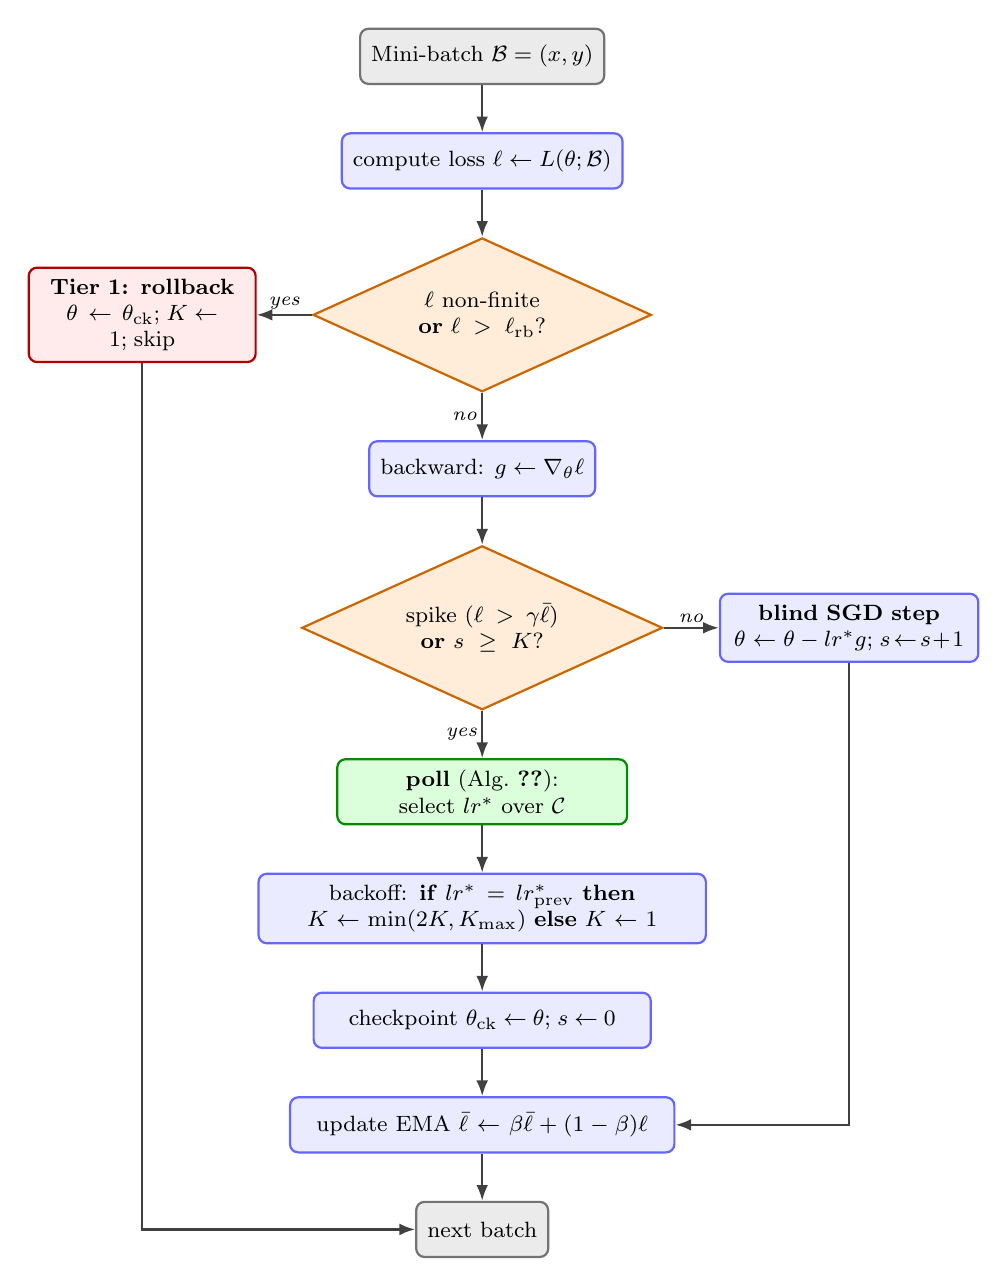
\begin{tikzpicture}[node distance=6mm and 7mm, flowfont]
  \node[startstop] (b) {Mini-batch $\mathcal{B}=(x,y)$};
  \node[proc, below=of b] (loss) {compute loss $\ell \leftarrow L(\theta;\mathcal{B})$};
  \node[decide, below=of loss, text width=28mm] (d1) {$\ell$ non-finite \textbf{or} $\ell > \ell_{\mathrm{rb}}$?};
  \node[guard, left=of d1, text width=26mm] (rb) {\textbf{Tier 1: rollback}\\$\theta \leftarrow \theta_{\mathrm{ck}}$;\;$K\!\leftarrow\!1$;\;skip};
  \node[proc, below=of d1] (grad) {backward: $g \leftarrow \nabla_\theta \ell$};
  \node[decide, below=of grad, text width=30mm] (d2) {spike ($\ell > \gamma\bar\ell$)\\\textbf{or} $s \ge K$?};
  \node[proc, right=of d2, text width=30mm] (blind) {\textbf{blind SGD step}\\$\theta \leftarrow \theta - lr^{*} g$;\;$s\!\leftarrow\!s\!+\!1$};
  \node[pick, below=of d2, text width=34mm] (poll) {\textbf{poll} (Alg.~\ref{alg:polling}):\\select $lr^{*}$ over $\mathcal{C}$};
  \node[proc, below=of poll, text width=54mm] (back) {backoff: \textbf{if} $lr^{*}\!=\!lr^{*}_{\mathrm{prev}}$ \textbf{then} $K\!\leftarrow\!\min(2K,K_{\max})$ \textbf{else} $K\!\leftarrow\!1$};
  \node[proc, below=of back, text width=40mm] (ck) {checkpoint $\theta_{\mathrm{ck}}\!\leftarrow\!\theta$;\;$s\!\leftarrow\!0$};
  \node[proc, below=of ck, text width=46mm] (ema) {update EMA $\bar\ell \leftarrow \beta\bar\ell+(1-\beta)\ell$};
  \node[startstop, below=of ema] (next) {next batch};
  \draw[flowarr] (b) -- (loss);
  \draw[flowarr] (loss) -- (d1);
  \draw[flowarr] (d1) -- node[flbl,left]{no} (grad);
  \draw[flowarr] (d1) -- node[flbl,above]{yes} (rb);
  \draw[flowarr] (grad) -- (d2);
  \draw[flowarr] (d2) -- node[flbl,above]{no} (blind);
  \draw[flowarr] (d2) -- node[flbl,left]{yes} (poll);
  \draw[flowarr] (poll) -- (back);
  \draw[flowarr] (back) -- (ck);
  \draw[flowarr] (ck) -- (ema);
  \draw[flowarr] (ema) -- (next);
  \draw[flowarr] (blind.south) |- (ema.east);
  \draw[flowarr] (rb.south) |- (next.west);
\end{tikzpicture}%
}
\caption{Control flow of one Efficient Polling batch (Algorithm~\ref{alg:efficient}). Most batches take the cheap \emph{blind SGD step} (right); a poll is forced only when the interval elapses ($s \ge K$) or a loss spike is detected, after which exponential backoff grows or resets the polling interval $K$. The two-tier divergence guard intercepts broken weights (Tier~1, left, which skips to the next batch) and suspicious spikes (Tier~2, via the poll). Each poll also refreshes the rollback checkpoint $\theta_{\mathrm{ck}}$.}
\label{fig:eff-flow}
\end{figure}

\section{Experiments}

\subsection{Experimental Setup}

All experiments use CIFAR-10~\cite{krizhevsky2009cifar}, consisting of 50{,}000 training and 10{,}000 test images across 10 classes ($32\!\times\!32$ RGB). The full implementation is publicly available in the project repository.\footnote{\url{https://github.com/luiz-linkezio/Efficient-Polling-Based-Learning-Rate-Optimization-for-Neural-Networks}} We reserve 10\% of training data for validation, yielding 45{,}000 training and 5{,}000 validation images.

The model, \texttt{SimpleCIFAR10CNN}, is a five-layer CNN with the following structure: two blocks each consisting of two convolutional layers (64 and 128 channels, $3\!\times\!3$ kernels, ReLU activations, MaxPool downsampling), a third block with one 256-channel convolutional layer followed by AdaptiveAvgPool$(1\!\times\!1)$, and a Linear$(256, 10)$ classification head. The network has $557{,}898$ trainable parameters ($\approx 0.56$\,M), and uses no batch normalization or dropout, so that the optimizer is the only source of adaptation under study.

Images are normalized per channel using training set statistics (RGB means: $[125.31,\, 122.95,\, 113.87]$; stds: $[62.99,\, 62.09,\, 66.70]$). All methods use vanilla SGD (no momentum, no weight decay) as the base optimizer with batch size 64 and 150 epochs. With 45{,}000 training images and batch size 64, each epoch comprises $704$ batches, for a total of $105{,}600$ batches over the full run. The base learning rate is $10^{-3}$ for all methods. A single random seed (42) is fixed for weight initialization, data shuffling, and the train/validation split, so that the three methods differ only in their learning-rate selection logic and all results below come from one fully reproducible run per method. Wall-clock timings were measured on a single NVIDIA GeForce RTX 5070 (12\,GB) with no other GPU workload.

\subsection{Baseline Replication}

The baseline applies SGD with a fixed learning rate of $10^{-3}$ throughout all 150 epochs. As shown in Fig.~\ref{fig:losses}, validation loss decreases monotonically and accuracy improves steadily, achieving 57.28\% best validation accuracy and 56.70\% test accuracy. The conservative fixed LR ensures stable, predictable convergence and provides a clean reference point.

\subsection{Polling Method Replication}

The primary experimental goal of this work is to replicate the Polling Method of Tan et al.\ in a new setting. The original paper evaluated it on MNIST with a two-layer ANN and candidate LRs in $[0.01, 0.05]$. Our replication targets CIFAR-10, a harder 10-class benchmark, using a CNN (\texttt{SimpleCIFAR10CNN}) and vanilla SGD with candidate LRs spanning five orders of magnitude ($10^{-5}$ to $10^{-1}$). Despite differences in architecture, dataset, and candidate LR range, the core algorithm is preserved exactly: at each batch, $N$ independent weight updates are evaluated and the one with highest batch accuracy is kept. The replication result (84.65\% best validation accuracy, 83.99\% test accuracy) demonstrates that the polling selection mechanism successfully discovers a two-phase LR schedule entirely from batch-level feedback, without any prior knowledge of the optimal rate.

\section{Results}

Table~\ref{tab:results} summarizes the performance of all three methods and Table~\ref{tab:cost} their computational cost. Fig.~\ref{fig:losses} shows training and validation loss curves and Fig.~\ref{fig:lrs} shows the learning rate trajectories across all 150 epochs.

\begin{table}[htbp]
\caption{Performance Comparison Across Methods (150 Epochs)}
\begin{center}
\resizebox{\columnwidth}{!}{%
\begin{tabular}{|l|c|c|c|}
\hline
\textbf{Method} & \textbf{Best Val} & \textbf{Test Acc} & \textbf{Test Loss} \\
\hline
Baseline                     & 57.28\%          & 56.70\%          & 1.2155 \\
Polling (base paper) & 84.65\%        & \textbf{83.99\%} & \textbf{0.6832} \\
\textbf{Efficient Polling}   & \textbf{85.07\%} & 83.93\%          & 0.7319 \\
\hline
\end{tabular}%
}
\end{center}
\label{tab:results}
\end{table}

\begin{table}[htbp]
\caption{Computational Cost (150 Epochs, 105{,}600 Batches)}
\begin{center}
\resizebox{\columnwidth}{!}{%
\begin{tabular}{|l|c|c|c|}
\hline
\textbf{Method} & \textbf{Polled Batches} & \textbf{Optimizer Steps} & \textbf{s/Epoch} \\
\hline
Baseline          & ---            & 105{,}600          & 2.50 \\
Polling (base paper) & 100\%  & 528{,}000          & 9.10 \\
\textbf{Efficient Polling} & \textbf{5.05\%} & \textbf{132{,}285} & \textbf{2.79} \\
\hline
\end{tabular}%
}
\end{center}
\label{tab:cost}
\end{table}

\begin{figure}[htbp]
\centerline{
\includegraphics[width=\columnwidth]{images/training_comparison_losses.png}}
\caption{Training and validation loss over 150 epochs for all three methods. Both the Polling and Efficient Polling methods converge rapidly and achieve low validation loss, significantly outperforming the baseline. Efficient Polling closely tracks the base method's trajectory despite polling only 5\% of batches. The baseline converges slowly under the fixed conservative LR.}
\label{fig:losses}
\end{figure}

\begin{figure}[htbp]
\centerline{
\includegraphics[width=\columnwidth]{images/training_comparison_LRs.png}}
\caption{Mean selected learning rate per epoch for all three methods (symlog scale). The Polling method autonomously selects the highest candidate (${\approx}\,10^{-1}$) for the first ${\approx}\,36$ epochs, then transitions abruptly to the smallest candidate (${\approx}\,10^{-5}$) as the model converges. Efficient Polling recovers the same two-phase schedule (high LR until ${\approx}$ epoch 36, annealing to $10^{-5}$ by ${\approx}$ epoch 67) while polling only a small fraction of batches. The baseline remains constant at $10^{-3}$.}
\label{fig:lrs}
\end{figure}

The Polling Method achieves 84.65\% best validation accuracy and 83.99\% test accuracy, outperforming the baseline by ${\approx}\,27$ percentage points. As shown in Fig.~\ref{fig:lrs}, the mean selected LR rapidly converges to ${\approx}\,10^{-1}$ and remains there through the first ${\approx}\,36$ epochs, enabling rapid loss reduction visible in Fig.~\ref{fig:losses}. After this aggressive exploration phase, the selected LR collapses to the smallest candidate (${\approx}\,10^{-5}$), facilitating fine-grained refinement near convergence.

The Efficient Polling method achieves 85.07\% best validation accuracy and 83.93\% test accuracy, matching the base Polling method within 0.1 pp on test accuracy and slightly exceeding it on validation, while polling only 5{,}337 of 105{,}600 batches (5.05\%). As shown in Fig.~\ref{fig:lrs}, it recovers the same two-phase schedule as base Polling: the highest candidate dominates the first ${\approx}\,36$ epochs, after which the selection anneals to the smallest candidate by ${\approx}$ epoch 67. As summarized in Table~\ref{tab:cost}, the on-demand schedule reduces total optimizer steps from 528{,}000 to 132{,}285 (75\% fewer) and wall-clock time from 9.10 to 2.79\,s per epoch ($3.3\times$ faster), only 12\% above plain SGD.\footnote{Wall-clock times were measured in isolated 3-epoch runs to avoid GPU warm-up and cross-method contention; accuracy and loss figures are taken from the single, fully reproducible 150-epoch run reported throughout this section.} The divergence guard remained cheap to invoke: across all 5{,}337 polls, not a single rollback to a checkpoint was triggered, indicating that the spike-triggered tier alone was sufficient to intercept unstable steps before they were applied. Its necessity is nonetheless demonstrated by an unguarded preliminary run, in which a single blind step at $lr = 10^{-1}$ around epoch 33 pushed the weights into numerical divergence (NaN loss), from which the unguarded method could not recover for the remaining 117 epochs.

\subsection{Computational Cost Model}
\label{sec:cost}

The cost of each method follows directly from how often it polls. Base Polling executes $N = 5$ trial updates on every one of the $105{,}600$ batches, for $528{,}000$ optimizer steps. Efficient Polling instead pays the polling cost only on polled batches. Each poll performs $N$ trial updates plus one re-application of the winning step ($N + 1 = 6$ steps), while each unpolled batch performs a single blind step. With $P = 5{,}337$ polls observed over the run,
\begin{equation}
S_{\mathrm{eff}} = P\,(N+1) + (B - P) = 5{,}337 \cdot 6 + 100{,}263 = 132{,}285,
\label{eq:cost}
\end{equation}
where $B = 105{,}600$ is the total number of batches, exactly reproducing the optimizer-step count in Table~\ref{tab:cost}. Polling therefore accounts for only $5{,}337 \cdot 6 = 32{,}022$ of the $132{,}285$ steps (24\%); the remaining 76\% are ordinary SGD steps, which is why per-epoch wall-clock time sits close to the plain-SGD baseline.

The poll count is itself a consequence of the exponential backoff. Once the selection stabilizes, the interval $K$ grows geometrically until it saturates at $K_{\max} = 64$, after which the method polls roughly once every $K_{\max}$ batches: $704 / 64 \approx 11$ polls per epoch. Fig.~\ref{fig:polls} confirms this behavior empirically. Outside the phase transition the per-epoch poll count tracks the $\approx 11$ steady-state floor closely, with brief geometric ramp-ups ($1, 2, 4, \ldots, 64$, at most $\log_2 K_{\max} = 6$ extra polls) whenever a poll momentarily disagrees. The transition itself is starkly visible: polling peaks at $233$ polls in epoch~33, the exact epoch at which the selected LR collapses from $10^{-1}$ to $10^{-5}$ (Fig.~\ref{fig:lrs}), because consecutive polls disagree and repeatedly reset $K$ to $1$. The polls thus concentrate precisely where the schedule changes and the selection actually carries information, which is the mechanism that lets $5\%$ of the batches recover the full two-phase schedule.

\begin{figure}[htbp]
\centerline{
\includegraphics[width=\columnwidth]{images/polls_per_epoch.png}}
\caption{Number of polls performed by Efficient Polling in each epoch (log scale). Outside the phase transition the count stays near the steady-state floor of $704/K_{\max} \approx 11$ polls per epoch (dashed line), the rate at which the saturated backoff interval forces a poll. Polling spikes to $233$ in epoch~33, the moment the selected LR transitions from $10^{-1}$ to $10^{-5}$, when disagreeing polls repeatedly reset the interval to one. Across the entire run only $5{,}337$ of $105{,}600$ batches (5.05\%) are polled, and no rollback is ever triggered.}
\label{fig:polls}
\end{figure}

\section{Discussion}

\subsection{Polling as Effective LR Discovery}

The Polling Method's dramatic improvement over the baseline (83.99\% vs.\ 56.70\% test accuracy) demonstrates that batch-level LR selection can autonomously discover a near-optimal two-phase schedule. In the first ${\approx}\,36$ epochs, the method consistently selects the highest candidate LR ($10^{-1}$), driving rapid loss reduction that the fixed-baseline SGD ($10^{-3}$) cannot match. The subsequent transition to the smallest candidate ($10^{-5}$) mirrors classical warm-up-then-decay schedules, but is derived entirely from batch accuracy feedback without any prior knowledge. This confirms that the optimal LR for vanilla SGD on CIFAR-10 lies far above the conservative value ($10^{-3}$) that would typically be chosen as a fixed rate, and that polling's candidate set must span the optimal region for the method to succeed.

\subsection{Efficient Polling: Same Schedule at a Fraction of the Cost}

The Efficient Polling results show that the value of polling lies in \emph{when the selection changes}, not in the selection itself being repeated at every batch. Within each phase of training the poll outcome is essentially constant (the highest candidate during exploration, the smallest near convergence), so the exponential backoff quickly settles at the maximum interval and the method degenerates into plain SGD at the discovered rate. Per-batch polling resumes automatically and only where it matters: during the phase transition, when consecutive polls disagree and the interval collapses back to one. This adaptivity is what allows 5\% of the polls to recover the full two-phase schedule, matching base Polling's accuracy at near-SGD cost.

The two methods leave the high-LR phase at the same point (the mean selected LR in both drops below $10^{-2}$ at epoch~37), but they anneal at different speeds. Base Polling, which re-decides every batch, collapses to the smallest candidate within about six epochs (reaching $\approx 10^{-5}$ by epoch~43), whereas Efficient Polling anneals more gradually and stabilizes at $10^{-5}$ only around epoch~67. This is a direct consequence of backoff: during the transition the polling interval has not yet reset to one for every batch, so the downward LR adjustments are applied at a coarser granularity. Crucially, this slower anneal costs nothing in final quality (Efficient Polling still reaches 100\% training accuracy by epoch~61 and slightly exceeds base Polling on validation), which indicates that the precise trajectory through the transition is far less important than reaching the high-LR regime early and the low-LR regime eventually. The persistent gap between perfect training accuracy and $\approx 85\%$ validation accuracy is shared by both polling methods, confirming that it reflects the capacity of the compact CNN rather than any instability introduced by sparse polling.

The divergence guard addresses the one genuine risk introduced by skipping polls. Base Polling implicitly validates every step before keeping it, so an explosive step at $lr = 10^{-1}$ is simply not selected; blind steps between polls have no such protection, and our unguarded preliminary run demonstrates that a single such step can irrecoverably destroy training. The guard restores the missing protection at negligible cost by reusing quantities the method already computes: the pre-step batch loss (for spike detection) and the poll-point state snapshots (as rollback checkpoints). Notably, the preventive tier alone was sufficient in practice: polling suspicious batches before stepping meant the recovery tier was never triggered in the guarded runs.

\subsection{Trade-offs}

\begin{itemize}
\item \textbf{Computational cost:} Base Polling requires $N = 5$ trial updates per batch, raising wall-clock time per epoch by $3.6\times$ over plain SGD. Efficient Polling reduces this overhead to 12\% over plain SGD (Table~\ref{tab:cost}) while preserving accuracy, making polling practical for routine use.
\item \textbf{Stability:} The fixed baseline is the most predictable. Base Polling is intrinsically safe because every step is validated before being kept. Efficient Polling trades this per-step validation for speed and recovers safety through its two-tier guard; without the guard, blind high-LR steps can diverge irrecoverably, as observed empirically.
\item \textbf{Generalization:} Both polling-based methods generalize well (test accuracy is within 0.66 pp of validation best for Polling and 1.14 pp for Efficient Polling), confirming that the polling selection criterion does not induce overfitting when applied per batch. The critical factor is ensuring the candidate set spans LR values near the true optimum for the given architecture and dataset.
\item \textbf{Hyperparameters:} Efficient Polling introduces four constants ($K_{\max}$, $\gamma$, $\beta$, $\ell_{\mathrm{rb}}$). None required tuning in our experiments: they encode scale-free heuristics (geometric backoff, relative loss spikes, random-guess loss) rather than problem-specific magnitudes.
\end{itemize}

\subsection{Limitations and Future Work}

Our conclusions rest on a single architecture, dataset, and base optimizer (vanilla SGD on CIFAR-10), and on one reproducible run per method rather than a multi-seed study; the absolute accuracies and the exact poll count would vary across seeds, even though the qualitative two-phase behavior is robustly driven by the candidate set. The method also presupposes that the candidate set $\mathcal{C}$ brackets the optimal LR: a candidate set that misses the optimal region would limit both polling variants regardless of polling frequency. Finally, the divergence guard reuses the per-batch loss and so assumes that loss spikes are a reliable proxy for impending divergence; this held throughout our runs (the recovery tier never fired), but pathological landscapes could in principle defeat the preventive tier. Natural extensions include combining polling with momentum or adaptive optimizers such as Adam, where the interaction between polled LR selection and per-parameter scaling is non-trivial, and evaluating on deeper networks and larger benchmarks where the cost savings of on-demand polling compound.

\section{Conclusion}

We replicated the Polling Method of Tan et al.\ on CIFAR-10, a setting that differs from the original in architecture (CNN vs.\ ANN), dataset, and candidate range, and confirmed that batch-level learning-rate selection autonomously discovers a near-optimal two-phase schedule, raising test accuracy from the baseline's 56.70\% to 83.99\% without any hand-designed LR formula. We then identified and removed the method's central weakness, its $N\times$ per-batch overhead, with the proposed Efficient Polling method. By polling on demand under an exponential-backoff schedule and protecting the unpolled steps with a two-tier divergence guard, Efficient Polling matches the base method's accuracy (83.93\% test, within 0.1 pp) while polling only 5.05\% of batches, cutting optimizer steps by 75\% and per-epoch wall-clock time by $3.3\times$ to within 12\% of plain SGD. The cost model of Eq.~\eqref{eq:cost} and the poll distribution of Fig.~\ref{fig:polls} together explain why: the value of polling lies in detecting \emph{when} the optimal LR changes, not in re-deciding it at every batch, and that detection is cheap. These results suggest that polling-based selection can be made practical for routine training, turning an accurate-but-expensive technique into one whose cost is essentially that of the underlying optimizer.

\begin{thebibliography}{00}
\bibitem{tan2025polling} R.~K. Tan, Z.~J. Choong, and M.~Lau, ``Expediting convergence via polling optimisation for gradient descent in neural networks,'' \emph{Journal of Experimental and Theoretical Analyses}, vol.~4, no.~1, art.~1, 2025.
\bibitem{kingma2015adam} D.~P. Kingma and J.~Ba, ``Adam: A method for stochastic optimization,'' in \emph{Proc. Int. Conf. Learning Representations (ICLR)}, 2015.
\bibitem{tieleman2012rmsprop} T.~Tieleman and G.~Hinton, ``Lecture 6.5---RMSProp: Divide the gradient by a running average of its recent magnitude,'' COURSERA: Neural Networks for Machine Learning, 2012.
\bibitem{loshchilov2017sgdr} I.~Loshchilov and F.~Hutter, ``SGDR: Stochastic gradient descent with warm restarts,'' in \emph{Proc. Int. Conf. Learning Representations (ICLR)}, 2017.
\bibitem{smith2017cyclical} L.~N. Smith, ``Cyclical learning rates for training neural networks,'' in \emph{Proc. IEEE Winter Conf. Applications of Computer Vision (WACV)}, 2017, pp. 464--472.
\bibitem{krizhevsky2009cifar} A.~Krizhevsky, ``Learning multiple layers of features from tiny images,'' Dept. Comput. Sci., Univ. of Toronto, Toronto, ON, Canada, Tech. Rep., 2009.
\bibitem{paszke2019pytorch} A.~Paszke, S.~Gross, F.~Massa, A.~Lerer, J.~Bradbury, G.~Chanan, \emph{et al.}, ``PyTorch: An imperative style, high-performance deep learning library,'' in \emph{Advances in Neural Information Processing Systems (NeurIPS)}, vol.~32, 2019.
\end{thebibliography}

\end{document}
